% Created 2018-07-01 周日 12:31
% Intended LaTeX compiler: XeLaTeX
\documentclass[a4paper, oneside, 11pt, UTF8]{ctexart}
\usepackage{my}

\begin{document}
\begin{titlepage}
	\centering
	
\includegraphics[width=0.15\textwidth]{image/lion.jpg}\par\vspace{1cm}
	\centering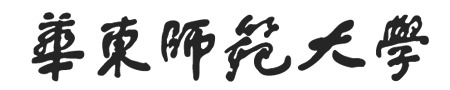
\includegraphics[width=0.9\textwidth]{image/logo-ecnu.jpg} \par
	\vspace{1cm}
	{\scshape\Large 儿童发展理论(双语)\par}
	\vspace{1.5cm}
	{\huge\bfseries 小班女孩心理自我防御机制行为的具体表现及分析\par}
	\vspace{2cm}
	{\Large\itshape 张亚栋\\10154508169\par}
	\vfill
	感谢\par
	\textbf{中国福利会幼儿园}\\上海市杨浦区国晓路300号

	\vfill

% Bottom of the page
% 	{\large \today\par} % 2018.7.1
	\zhdate{2018/7/1}
\end{titlepage}
\setcounter{page}{1} % new page
 \textbf{心理防御机制}\footnote{\href{http://wiki.mbalib.com/wiki/\%E5\%BF\%83\%E7\%90\%86\%E9\%98\%B2\%E5\%BE\%A1\%E6\%9C\%BA\%E5\%88\%B6}{心理防御机制-MBA智库百科}}是\textit{弗洛伊德} \includesvg[scale=0.3]{image/FreudSignature.svg}提出的心理学名词,是指自我对本我的压抑,这种压抑是自我的一种全然潜意识的自我防御功能。

 主要分为以下几种表现:
\begin{enumerate}
    \item 逃避机制:
        
        \begin{enumerate*}[label={\arabic*)},font={\color{cyan!50!black}\bfseries}]
            \item 压抑
            \item 否定
            \item 退行
            \item 潜抑
        \end{enumerate*}
    \item 自骗机制: 
    
        \begin{enumerate*}[label={\arabic*)},font={\color{cyan!50!black}\bfseries}]
            \item 反向
            \item 合理化
            \item 仪式抵消
            \item 隔离
            \item 理想化
            \item 分裂
        \end{enumerate*}
    \item 攻击机制:
    
        \begin{enumerate*}[label={\arabic*)},font={\color{cyan!50!black}\bfseries}]
            \item 转移
            \item 投射
        \end{enumerate*}
    \item 代替机制:
    
        \begin{enumerate*}[label={\arabic*)},font={\color{cyan!50!black}\bfseries}]
            \item 幻想 
            \item 补偿
        \end{enumerate*}
    \item 建设机制:
    
        \begin{enumerate*}[label={\arabic*)},font={\color{cyan!50!black}\bfseries}]
            \item 认同 
            \item 升华
        \end{enumerate*}
\end{enumerate}   
\par
弗洛伊德的理论一定程度上是无法通过实验进行验证的,只是提供了一种解释儿童行为和心理问题的经验化的归纳总结,能在个体问题上说得通,就算是其理论的成功应用。

\begin{tcolorbox}[enhanced,attach boxed title to top center={yshift=-3mm,yshifttext=-1mm},
  colback=blue!5!white,colframe=blue!75!black,colbacktitle=red!80!black,
  title=案例,fonttitle=\bfseries, fontupper=\CTEXindent,
  boxed title style={size=small,colframe=red!50!black}]
现在是小班的第二学期,老师鼓励幼儿一起分享交流,合作游戏。某次个别化活动时,其他小朋友都三三两两聚在一起活动,因为每个区可以是2  - 4名幼儿,唯独有个小女孩坐在画布前画画,我就走过去问她:你在画什么?她,没有回答我,继续在忙自己的画,正好带班老师在一旁看到,便跟我讲,这个小女孩是不爱说话。我就也没有继续问,心想可能也有小女孩跟我不太熟的原因。\par
研习的时候是每天都待在幼儿园的,所以有机会就可以看到小班的一日常规活动。我特别观察了小女孩,发现她确实不爱说话。每次到玩具时间,其他小朋友都在交换玩具,她却不会主动找其他
小朋友交换,别人交换过去的玩具她也不说自己要交换回来,就直接拿过来了。后来发现她有一个习惯就是别人跟她讲话,她
总回答“\pinyin{jiao1 jiao1}”,有时也不会去跟老师打招呼。我没懂这个“\pinyin{jiao1 jiao1}”是什么,别的小朋友也不知道她在说什么。带班老师的回答是,妈妈来接她的时候,她话很多的,到幼儿园里就是这样。另外,她还会去吸吮手指,或者手里拿到什么东西都往嘴里塞,在我见习结束时她都一直保持这个状态。
\end{tcolorbox}

%\clearpage


用弗洛伊德的理论来解释的话,上述小女孩的情况应该属于第 1 种:逃避机制。\par
具体来讲,小女孩可能是之前在幼儿园有过不愉快的经历,或者看到了什么自己不能接受的事件,就拒绝在幼儿园生活,失去了对班级的归属感,从而把这件事压制到自己的潜意识当中,从而不由自主地表现出一系列反常行为。\par
最明显的就是小女孩会去吸吮自己的手指,在家里面她不会这样做的,只是在幼儿园里出现这样的动作。通过几周的观察来看,这是一种比较消极的防御措施,只能暂时缓解她心理上的压抑,并不解决根本问题。另外,她总喜欢说\pinyin{“jiao1 jiao1”},以一种“掩耳盗铃”式的方式来回应他人,有一定的自我中心意识存在,毕竟还是在小班,幼儿园的去自我中心的管理方式对她的作用不大。\par
带班老师的管理风格偏向顺其自然,不用堵而是引导的方式来进行与幼儿沟通,我觉得这是一种比较有效和尊重幼儿的方式。虽然小女孩现在表现出了一些行为问题,但是慢慢长大的过程中这些问题会逐渐减缓的,过度的重视只会引起小女孩心理上更严重的疾病。
\end{document}
